\subsection{Map coloring}

\renewcommand{\CURPATH}{color/map}

It's possible to color all countries on any political map (or planar graph) using only 4 colors.

Any map or vertices on a planar graph can be colored using at most 4 colors.
This is quite interesting story behind this.
This is a first serious proof finished using automated theorem prover (Coq):
\url{https://en.wikipedia.org/wiki/Four_color_theorem}.

An example where I use graph coloring: \ref{tiling_Z3}.

Let's try to color map of Europe:

\lstinputlisting[style=custompy]{\CURPATH/1.py}

The output is to be fed to Wolfram Mathematica -- I'm using it to draw a map
\footnote{I copypasted pieces of it from \url{https://www.wolfram.com/mathematica/new-in-10/entity-based-geocomputation/find-a-four-coloring-of-a-map-of-europe.html}}:

\lstinputlisting{\CURPATH/1.txt}

\begin{figure}[H]
\centering
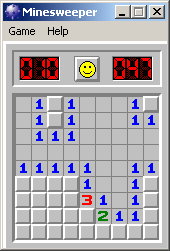
\includegraphics[scale=0.75]{\CURPATH/1.png}
\caption{Colored map}
\end{figure}

\subsubsection{MaxSMT or optimization problem}

Now let's have fun.
Out of pure whim, we may want to make as many countries colored as red as possible
\footnote{I took this idea from \url{https://www.cs.cmu.edu/~bryant/boolean/macgregor.html}}:

\begin{lstlisting}
s=Optimize()

...

s.maximize(Sum(*[If(country_color[i]==0, 1, 0) for i in range(countries_total)]))
\end{lstlisting}

\begin{figure}[H]
\centering
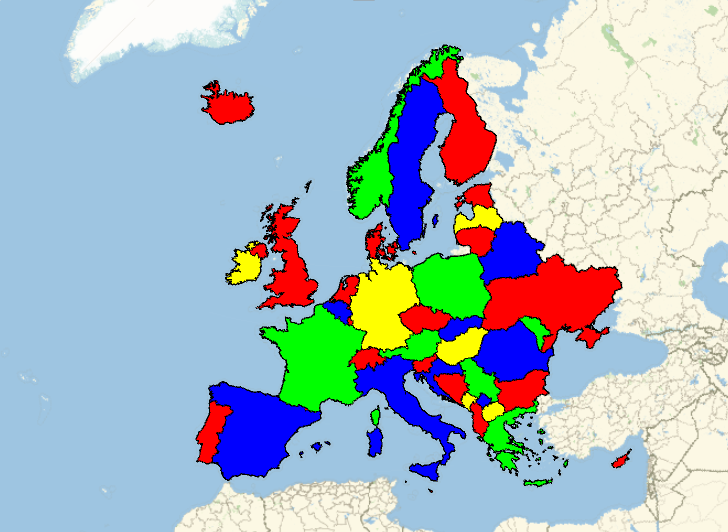
\includegraphics[scale=0.75]{\CURPATH/2_max_red.png}
\caption{The map}
\end{figure}

\lstinputlisting[caption=Statistics]{\CURPATH/2_max_red_stat.txt}

Or maybe we have a shortage of red paint?

\begin{lstlisting}
s.minimize(Sum(*[If(country_color[i]==0, 1, 0) for i in range(countries_total)]))
\end{lstlisting}

\begin{figure}[H]
\centering
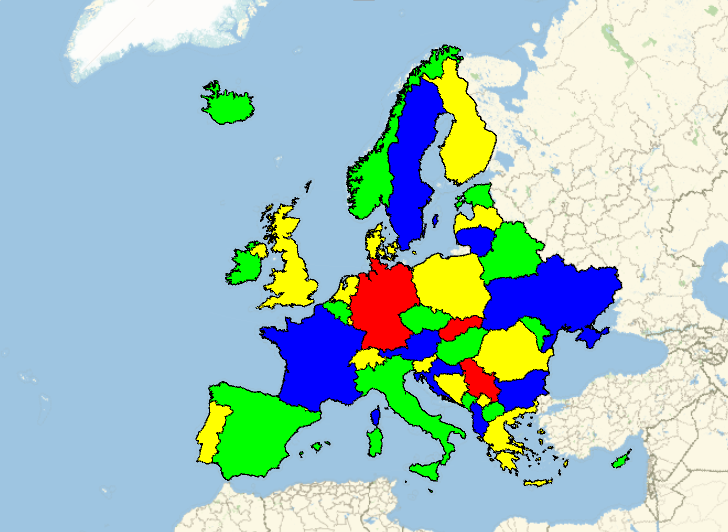
\includegraphics[scale=0.75]{\CURPATH/2_min_red.png}
\caption{The map}
\end{figure}

\lstinputlisting[caption=Statistics]{\CURPATH/2_min_red_stat.txt}

Two colors can be minimized/maximized simultaneously:

\begin{lstlisting}
...
s.minimize(Sum(*[If(Or(country_color[i]==0, country_color[i]==1), 1, 0) for i in range(countries_total)]))
...
\end{lstlisting}

